\documentclass[11pt,a4paper]{article}

% Packages
\usepackage[margin=2.5cm]{geometry}
\usepackage{microtype}
\usepackage{graphicx}
\usepackage{tikz}
\usetikzlibrary{shapes,arrows.meta,positioning,calc,fit,backgrounds,shadows.blur,decorations.pathmorphing,decorations.pathreplacing}
\usepackage{colortbl}
\usepackage{enumitem}
\usepackage{booktabs}
\usepackage{longtable}
\usepackage{hyperref}
\usepackage{xcolor}
\usepackage{fancyhdr}
\usepackage{titlesec}
\usepackage[most]{tcolorbox}
\usepackage{multicol}
\usepackage{amsmath,amssymb}
\usepackage{multirow}
\usepackage{setspace}
\usepackage{fontawesome5}
\usepackage{listings}

% Spacing
\setlength{\parskip}{3pt plus 1pt minus 1pt}
\setlength{\parindent}{0pt}

% Colors
\definecolor{primary}{HTML}{0E4D64}
\definecolor{secondary}{HTML}{137177}
\definecolor{accent}{HTML}{C84B31}
\definecolor{lightbg}{HTML}{E8F6F3}
\definecolor{defbg}{HTML}{FDF2E9}
\definecolor{greenhl}{HTML}{2E8B57}
\definecolor{purplehl}{HTML}{6C5B7B}
\definecolor{codebg}{HTML}{F4F6F7}

% Hyperref
\hypersetup{colorlinks=true, linkcolor=primary, urlcolor=secondary, citecolor=primary}

% Code listings style
\lstset{
  backgroundcolor=\color{codebg},
  basicstyle=\ttfamily\small,
  keywordstyle=\color{primary}\bfseries,
  stringstyle=\color{greenhl},
  commentstyle=\color{gray},
  breaklines=true,
  frame=l,
  framerule=2pt,
  rulecolor=\color{secondary!40},
  xleftmargin=8pt,
  framexleftmargin=6pt,
  aboveskip=6pt,
  belowskip=6pt
}

% Header/Footer
\pagestyle{fancy}
\fancyhf{}
\fancyhead[L]{\small\textcolor{primary}{\textbf{IoT for Data Science --- BSIT}}}
\fancyhead[R]{\small\textcolor{primary}{Lecture Handout}}
\fancyfoot[C]{\small\thepage}
\renewcommand{\headrulewidth}{0.5pt}
\renewcommand{\footrulewidth}{0.3pt}

% Section formatting
\titleformat{\section}{\Large\bfseries\color{primary}}{\thesection}{0.6em}{}[\vspace{2pt}\titlerule]
\titleformat{\subsection}{\large\bfseries\color{secondary}}{\thesubsection}{0.5em}{}
\titleformat{\subsubsection}{\normalsize\bfseries\color{primary}}{\thesubsubsection}{0.5em}{}
\titlespacing*{\section}{0pt}{14pt}{8pt}
\titlespacing*{\subsection}{0pt}{10pt}{5pt}

% Custom boxes
\newtcolorbox{definitionbox}[1][] {
  enhanced, breakable,
  colback=defbg, colframe=orange!60!black,
  colbacktitle=orange!70!black, coltitle=white,
  title={\faIcon{book}~#1}, fonttitle=\bfseries,
  boxrule=0pt, leftrule=4pt, arc=2pt,
  shadow={1mm}{-1mm}{0mm}{black!15},
  top=4pt, bottom=4pt, left=8pt, right=8pt
}
\newtcolorbox{conceptbox}[1][] {
  enhanced, breakable,
  colback=lightbg, colframe=secondary,
  colbacktitle=secondary, coltitle=white,
  title={\faIcon{lightbulb}~#1}, fonttitle=\bfseries,
  boxrule=0pt, leftrule=4pt, arc=2pt,
  shadow={1mm}{-1mm}{0mm}{black!15},
  top=4pt, bottom=4pt, left=8pt, right=8pt
}
\newtcolorbox{alertbox}[1][] {
  enhanced, breakable,
  colback=red!4, colframe=accent,
  colbacktitle=accent, coltitle=white,
  title={\faIcon{exclamation-triangle}~#1}, fonttitle=\bfseries,
  boxrule=0pt, leftrule=4pt, arc=2pt,
  shadow={1mm}{-1mm}{0mm}{black!12},
  top=3pt, bottom=3pt, left=8pt, right=8pt
}
\newtcolorbox{examplebox}[1][] {
  enhanced, breakable,
  colback=green!4, colframe=greenhl,
  colbacktitle=greenhl, coltitle=white,
  title={\faIcon{code}~#1}, fonttitle=\bfseries,
  boxrule=0pt, leftrule=4pt, arc=2pt,
  shadow={1mm}{-1mm}{0mm}{black!12},
  top=3pt, bottom=3pt, left=8pt, right=8pt
}

\begin{document}

% Title
\begin{center}
\vspace*{0.5cm}
{\Huge\bfseries\textcolor{primary}{IoT for Data Science}}\\[8pt]
{\Huge\bfseries\textcolor{primary}{Connected Systems Foundations}}\\[16pt]
{\color{secondary}\rule{0.68\textwidth}{1.5pt}}\\[12pt]
{\Large\textsc{BSIT Lecture Handout}}\\[6pt]
{\large\textcolor{gray!70!black}{Course: Data Science \quad Program: BSIT}}\\[8pt]
{\normalsize\textcolor{gray!70!black}{Sensors \textbullet\ Connectivity \textbullet\ Edge Computing \textbullet\ Protocols \textbullet\ Security}}
\vspace{0.3cm}
\end{center}

\tableofcontents
\newpage

%=============================================================
\section{Introduction to the Internet of Things}
%=============================================================

\begin{definitionbox}[Internet of Things]
The Internet of Things, or IoT, is a network of physical objects that can sense, process, communicate, and sometimes act on their environment. These objects include sensors, smart appliances, vehicles, wearable devices, industrial machines, and many other embedded systems connected through local or global networks.
\end{definitionbox}

\begin{conceptbox}[Why This Topic Appears in a Data Science Course]
IoT is included here because connected devices are major producers of real-world data. The focus of this handout is not data science algorithms. Instead, it explains how IoT systems are built, how devices communicate, how data moves through the system, and what technical issues must be solved before analytics can happen.
\end{conceptbox}

\subsection{Core Ideas Behind IoT}

\begin{itemize}[leftmargin=*]
  \item \textbf{Sensing:} Devices observe temperature, motion, pressure, location, light, sound, or other environmental conditions.
  \item \textbf{Connectivity:} Devices send telemetry to gateways, platforms, or peer devices through wired or wireless links.
  \item \textbf{Processing:} Data may be processed on the device, at the edge, or in the cloud.
  \item \textbf{Actuation:} Systems can trigger a response such as opening a valve, switching a relay, or sending an alarm.
  \item \textbf{Management:} Devices need configuration, authentication, updates, monitoring, and retirement over time.
\end{itemize}

\subsection{The Sense-to-Action Cycle}

\begin{center}
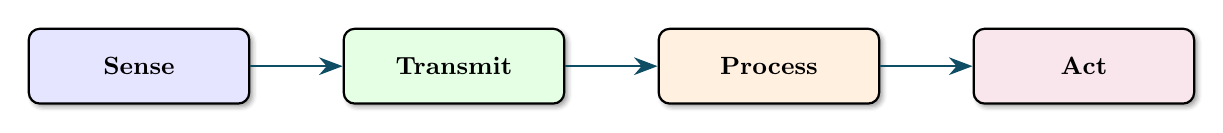
\begin{tikzpicture}[
  cycbox/.style={rectangle, draw, thick, rounded corners=4pt, minimum width=2.8cm, minimum height=0.95cm, align=center, font=\small\bfseries,
    blur shadow={shadow blur steps=4, shadow xshift=0.4mm, shadow yshift=-0.4mm}},
  arr/.style={-{Stealth[length=3mm]}, thick, primary}
]
  \node[cycbox, fill=blue!10] (sense) at (0,0) {Sense};
  \node[cycbox, fill=green!10] (transmit) at (4.0,0) {Transmit};
  \node[cycbox, fill=orange!12] (process) at (8.0,0) {Process};
  \node[cycbox, fill=purple!10] (act) at (12.0,0) {Act};

  \draw[arr] (sense) -- (transmit);
  \draw[arr] (transmit) -- (process);
  \draw[arr] (process) -- (act);
\end{tikzpicture}
\end{center}

\subsection{Common Characteristics of IoT Systems}

\begin{itemize}[leftmargin=*]
  \item Large numbers of devices working together.
  \item Small, resource-constrained hardware with limited CPU, memory, and power.
  \item Continuous or periodic data generation.
  \item Operation in changing physical environments.
  \item Dependence on secure identity, reliable communication, and long-term maintainability.
\end{itemize}

%=============================================================
\section{IoT Ecosystem and Architecture}
%=============================================================

\subsection{Typical IoT Architecture}

\begin{center}
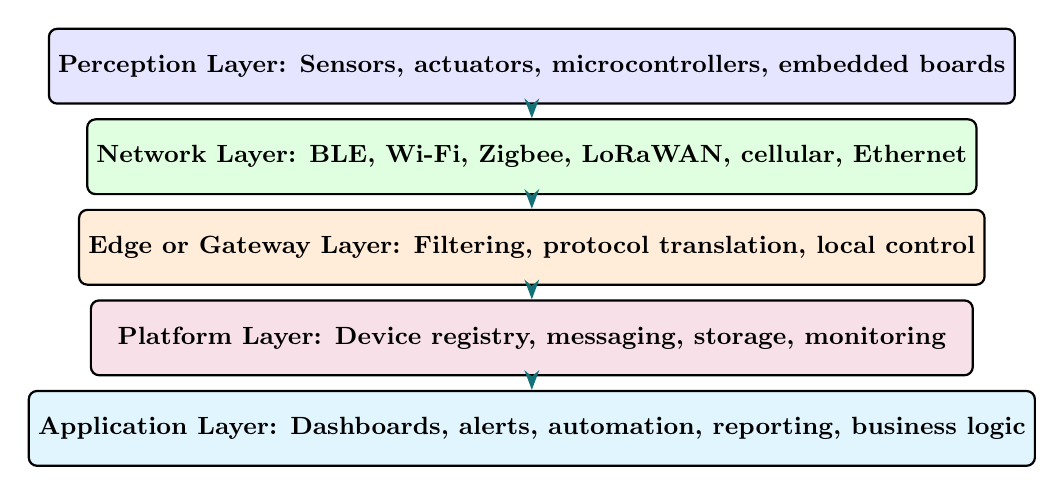
\begin{tikzpicture}[
  layer/.style={rectangle, draw, thick, minimum width=11.2cm, minimum height=0.95cm, align=center, font=\small\bfseries, rounded corners=3pt},
  arr/.style={-{Stealth[length=2.5mm]}, thick, secondary}
]
  \node[layer, fill=blue!10] (device) at (0,0) {Perception Layer: Sensors, actuators, microcontrollers, embedded boards};
  \node[layer, fill=green!12] (network) at (0,-1.15) {Network Layer: BLE, Wi-Fi, Zigbee, LoRaWAN, cellular, Ethernet};
  \node[layer, fill=orange!15] (edge) at (0,-2.3) {Edge or Gateway Layer: Filtering, protocol translation, local control};
  \node[layer, fill=purple!12] (platform) at (0,-3.45) {Platform Layer: Device registry, messaging, storage, monitoring};
  \node[layer, fill=cyan!12] (app) at (0,-4.6) {Application Layer: Dashboards, alerts, automation, reporting, business logic};

  \draw[arr] (device) -- (network);
  \draw[arr] (network) -- (edge);
  \draw[arr] (edge) -- (platform);
  \draw[arr] (platform) -- (app);
\end{tikzpicture}
\end{center}

\subsection{Main Components in the Ecosystem}

\begin{longtable}{p{3.0cm}p{4.2cm}p{5.6cm}}
\toprule
\textbf{Component} & \textbf{Role} & \textbf{Examples} \\
\midrule
End device & Observes or controls the physical world & Smart meter, wearable band, soil sensor, smart bulb \\
Gateway & Bridges local devices to wider networks and may preprocess data & Industrial gateway, home hub, edge computer \\
Communication network & Carries data between nodes and services & Wi-Fi, cellular, Zigbee mesh, Ethernet \\
IoT platform & Handles device identity, messaging, storage, commands, monitoring & Device registry, broker, telemetry dashboard \\
Application & Gives value to users through control panels, alerts, and automation & Smart campus app, predictive maintenance console \\
\bottomrule
\end{longtable}

\subsection{Centralized and Distributed Designs}

\begin{itemize}[leftmargin=*]
  \item \textbf{Centralized IoT:} Devices send most data to a cloud platform where decisions are made.
  \item \textbf{Distributed IoT:} More decisions happen near the devices through gateways or edge nodes.
  \item \textbf{Hybrid IoT:} Time-sensitive actions happen locally while long-term storage and fleet management happen centrally.
\end{itemize}

\begin{examplebox}[Architecture Choice]
A smart irrigation system may measure soil moisture in the field, let a local controller decide whether to open a valve, and still send summaries to a cloud dashboard for remote supervision.
\end{examplebox}

%=============================================================
\section{Sensors, Actuators, and Embedded Devices}
%=============================================================

\subsection{Sensors}

\begin{definitionbox}[Sensor]
A sensor is a device that converts a physical phenomenon into an electrical signal that can be measured and interpreted by a controller. Sensors are the main entry point of data into an IoT system.
\end{definitionbox}

\begin{longtable}{p{3.1cm}p{3.8cm}p{5.8cm}}
\toprule
\textbf{Sensor Type} & \textbf{Measures} & \textbf{Typical IoT Use} \\
\midrule
Temperature sensor & Heat level & Cold-chain tracking, HVAC systems, weather stations \\
Motion sensor & Movement or presence & Smart lighting, intrusion detection, occupancy tracking \\
Pressure sensor & Force per unit area & Industrial monitoring, vehicle systems, pipelines \\
Light sensor & Illumination level & Street lighting, greenhouse control, phone brightness \\
GPS module & Geographic position & Fleet tracking, asset monitoring, navigation \\
Gas sensor & Air quality or chemical presence & Safety systems, pollution monitoring, smart labs \\
\bottomrule
\end{longtable}

\subsection{Actuators}

\begin{definitionbox}[Actuator]
An actuator receives a command from the system and performs a physical action. If sensors represent input from the environment, actuators represent output back to the environment.
\end{definitionbox}

\begin{itemize}[leftmargin=*]
  \item Electric relays switch devices on or off.
  \item Motors create movement in robots, doors, pumps, and valves.
  \item Buzzers and lights produce alerts.
  \item Solenoid valves control flow in water or gas systems.
\end{itemize}

\subsection{Embedded Controllers and Device Constraints}

\begin{conceptbox}[Resource Constraints]
Unlike laptops or servers, many IoT devices have very limited memory, battery capacity, bandwidth, and processing power. Designers must therefore be careful about code size, communication overhead, power use, and update strategy.
\end{conceptbox}

\begin{multicols}{2}
\begin{itemize}[leftmargin=1.2em]
  \item Microcontrollers
  \item Single-board computers
  \item Real-time operating systems
  \item Battery-powered nodes
  \item Sleep and wake cycles
  \item Local buffering
\end{itemize}
\end{multicols}

\subsection{Calibration and Signal Quality}

\begin{alertbox}[Garbage In, Garbage Out]
If a sensor is poorly calibrated, badly placed, electrically noisy, or physically damaged, every higher layer of the IoT system is affected. Reliable IoT starts with correct sensing, not with dashboards.
\end{alertbox}

%=============================================================
\section{Connectivity and Communication Protocols}
%=============================================================

\subsection{Connectivity Options}

\begin{itemize}[leftmargin=*]
  \item \textbf{Wi-Fi:} High throughput for homes, buildings, and campuses, but relatively high power use.
  \item \textbf{Bluetooth Low Energy (BLE):} Short-range, low-power communication for wearables and personal devices.
  \item \textbf{Zigbee and Thread:} Low-power mesh networking for smart homes and building automation.
  \item \textbf{LoRaWAN:} Long-range, low-bandwidth communication for remote sensing and smart agriculture.
  \item \textbf{Cellular:} Wide-area coverage for vehicles, logistics, and mobile deployments.
  \item \textbf{Ethernet:} Stable wired option for industrial and fixed installations.
\end{itemize}

\subsection{Application Protocols}

\begin{longtable}{p{2.3cm}p{2.5cm}p{4.0cm}p{3.9cm}}
\toprule
\textbf{Protocol} & \textbf{Pattern} & \textbf{Strength} & \textbf{Typical Use} \\
\midrule
MQTT & Publish and subscribe & Lightweight messaging over unreliable links & Telemetry from constrained devices \\
HTTP & Request and response & Simple and widely supported & Web APIs, configuration portals \\
CoAP & Request and response & Designed for constrained devices and UDP transport & Low-power sensor nodes \\
AMQP & Message queues & Reliable enterprise messaging & Industrial integration, backend systems \\
\bottomrule
\end{longtable}

\subsection{Topics, Messages, and Payloads}

\begin{conceptbox}[Message Design]
IoT systems do not only need connectivity. They also need a message design: what is sent, how often it is sent, which device sent it, how the receiver interprets it, and what happens when messages arrive late, duplicated, or out of order.
\end{conceptbox}

\begin{examplebox}[MQTT Topic Example]
An MQTT topic such as \texttt{campus/buildingA/room204/temperature} lets subscribers receive only the telemetry they need. Topic naming helps organize large fleets of devices.
\end{examplebox}

\subsection{Network Tradeoffs}

\begin{itemize}[leftmargin=*]
  \item Long range often means lower data rate.
  \item Low power often means small payloads and less frequent transmission.
  \item High throughput often requires more energy and stronger infrastructure.
  \item Reliability may require acknowledgments, retries, buffering, or redundant paths.
\end{itemize}

%=============================================================
\section{Edge, Fog, and Cloud in IoT}
%=============================================================

\subsection{Where Processing Happens}

\begin{definitionbox}[Edge Computing]
Edge computing means processing data close to where it is generated, such as on the device itself or on a nearby gateway. This reduces latency, saves bandwidth, and can improve privacy.
\end{definitionbox}

\begin{definitionbox}[Fog Computing]
Fog computing is an intermediate model in which processing is distributed across local or regional infrastructure between the device layer and the cloud. It is useful when many nearby devices need coordination.
\end{definitionbox}

\subsection{Edge-to-Cloud Flow}

\begin{center}
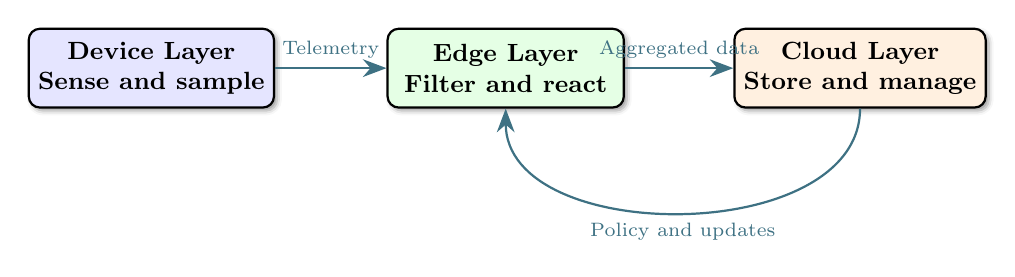
\begin{tikzpicture}[
  flowbox/.style={rectangle, draw, thick, rounded corners=4pt, minimum width=3.0cm, minimum height=1.0cm, align=center, font=\small\bfseries,
    blur shadow={shadow blur steps=3, shadow xshift=0.4mm, shadow yshift=-0.4mm}},
  arr/.style={-{Stealth[length=3mm]}, thick, primary!80}
]
  \node[flowbox, fill=blue!10] (device) at (0,0) {Device Layer\\Sense and sample};
  \node[flowbox, fill=green!10] (edge) at (4.5,0) {Edge Layer\\Filter and react};
  \node[flowbox, fill=orange!12] (cloud) at (9.0,0) {Cloud Layer\\Store and manage};

  \draw[arr] (device) -- node[above, font=\scriptsize] {Telemetry} (edge);
  \draw[arr] (edge) -- node[above, font=\scriptsize] {Aggregated data} (cloud);
  \draw[arr] (cloud.south) to[out=-90,in=-90] node[below, font=\scriptsize] {Policy and updates} (edge.south);
\end{tikzpicture}
\end{center}

\subsection{Why Edge Computing Matters in IoT}

\begin{itemize}[leftmargin=*]
  \item Local decisions can happen even when internet connectivity is weak or absent.
  \item Bandwidth costs are reduced because only summaries or events need to be transmitted.
  \item Sensitive raw data may stay closer to where it was generated.
  \item Time-critical systems such as robotics or safety alarms need low latency.
\end{itemize}

\subsection{When Cloud Still Matters}

\begin{itemize}[leftmargin=*]
  \item Fleet-wide device management.
  \item Long-term storage and compliance archives.
  \item Global dashboards and multi-site visibility.
  \item Centralized software update control.
  \item Integration with enterprise applications and identity services.
\end{itemize}

%=============================================================
\section{Device Lifecycle and IoT Data Flow}
%=============================================================

\subsection{From Provisioning to Retirement}

\begin{center}
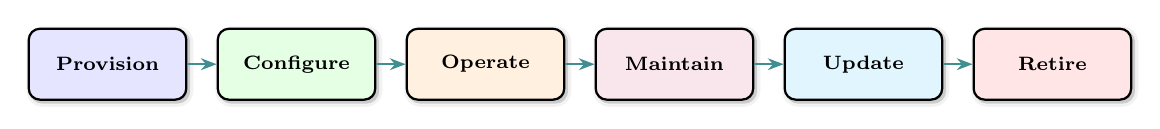
\begin{tikzpicture}[
  lifebox/.style={rectangle, draw, thick, rounded corners=4pt, minimum width=2.0cm, minimum height=0.9cm, align=center, font=\scriptsize\bfseries,
    blur shadow={shadow blur steps=2, shadow xshift=0.3mm, shadow yshift=-0.3mm}},
  arr/.style={-{Stealth[length=2mm]}, thick, secondary!80}
]
  \node[lifebox, fill=blue!10] (p1) at (0,0) {Provision};
  \node[lifebox, fill=green!10] (p2) at (2.4,0) {Configure};
  \node[lifebox, fill=orange!12] (p3) at (4.8,0) {Operate};
  \node[lifebox, fill=purple!10] (p4) at (7.2,0) {Maintain};
  \node[lifebox, fill=cyan!12] (p5) at (9.6,0) {Update};
  \node[lifebox, fill=red!10] (p6) at (12.0,0) {Retire};

  \draw[arr] (p1) -- (p2);
  \draw[arr] (p2) -- (p3);
  \draw[arr] (p3) -- (p4);
  \draw[arr] (p4) -- (p5);
  \draw[arr] (p5) -- (p6);
\end{tikzpicture}
\end{center}

\subsection{Lifecycle Stages}

\begin{itemize}[leftmargin=*]
  \item \textbf{Provisioning:} Register the device, assign credentials, and define identity.
  \item \textbf{Configuration:} Set sampling intervals, thresholds, network settings, and policy.
  \item \textbf{Operation:} Collect telemetry, receive commands, and monitor status.
  \item \textbf{Maintenance:} Replace batteries, recalibrate sensors, and repair hardware faults.
  \item \textbf{Firmware updates:} Deliver secure over-the-air updates to fix bugs or add features.
  \item \textbf{Retirement:} Revoke credentials, archive records, and safely remove the device from service.
\end{itemize}

\subsection{Telemetry, Events, and Commands}

\begin{longtable}{p{3.0cm}p{4.0cm}p{5.7cm}}
\toprule
\textbf{Message Type} & \textbf{Direction} & \textbf{Purpose} \\
\midrule
Telemetry & Device to platform & Periodic measurements such as temperature or battery level \\
Event & Device to platform & Report something meaningful such as a door opened or threshold exceeded \\
Command & Platform to device & Request an action such as restart, set fan speed, or open valve \\
Status report & Device to platform & Share health information such as uptime or firmware version \\
\bottomrule
\end{longtable}

\subsection{Digital Twins}

\begin{definitionbox}[Digital Twin]
A digital twin is a virtual representation of a physical device or asset. It stores the device state, desired configuration, and operational history so software can reason about the real object without direct physical access.
\end{definitionbox}

%=============================================================
\section{Security, Privacy, and Reliability in IoT}
%=============================================================

\subsection{Why IoT Security Is Difficult}

\begin{alertbox}[A Larger Attack Surface]
IoT security is harder than ordinary application security because the system includes hardware, firmware, radio communication, network services, cloud services, physical access risks, and long-lived devices that may remain deployed for years.
\end{alertbox}

\subsection{Common Security Risks}

\begin{itemize}[leftmargin=*]
  \item Default passwords or weak authentication.
  \item Unencrypted communication over insecure channels.
  \item Unsigned firmware updates or poorly protected boot processes.
  \item Insecure APIs exposing device control or telemetry.
  \item Physical tampering with field devices.
  \item Poor key storage on constrained hardware.
\end{itemize}

\subsection{Essential Security Controls}

\begin{itemize}[leftmargin=*]
  \item Unique device identity for every node.
  \item Mutual authentication between device and platform.
  \item Encryption in transit and secure storage for secrets.
  \item Secure boot and signed firmware updates.
  \item Least-privilege access for applications and operators.
  \item Logging, anomaly detection, and incident response procedures.
\end{itemize}

\subsection{Privacy and Ethics}

\begin{conceptbox}[Responsible Collection]
Many IoT systems observe people, movement, health, or behavior. Designers must therefore think about consent, data minimization, lawful use, retention limits, and the consequences of continuous monitoring.
\end{conceptbox}

\subsection{Reliability and Maintenance}

\begin{itemize}[leftmargin=*]
  \item Plan for packet loss, dead batteries, sensor drift, and unstable connectivity.
  \item Use retries, buffering, heartbeats, and watchdog timers where appropriate.
  \item Expect hardware failure and design for replacement.
  \item Measure uptime, signal quality, message delay, and battery health.
\end{itemize}

%=============================================================
\section{IoT Use Cases, Challenges, and BSIT Skills}
%=============================================================

\subsection{Representative IoT Use Cases}

\begin{itemize}[leftmargin=*]
  \item \textbf{Smart homes:} Lighting, security, energy monitoring, and appliance control.
  \item \textbf{Industrial IoT:} Machine monitoring, predictive maintenance, and process automation.
  \item \textbf{Smart agriculture:} Soil moisture sensing, weather monitoring, and irrigation control.
  \item \textbf{Healthcare IoT:} Wearables, remote patient monitoring, and medication tracking.
  \item \textbf{Smart cities:} Parking systems, traffic sensors, environmental monitoring, and smart bins.
  \item \textbf{Smart campuses:} Room occupancy, lab condition monitoring, access control, and utility tracking.
\end{itemize}

\subsection{Mini Case Study: Smart Classroom Monitoring}

\begin{examplebox}[Scenario]
A campus installs environmental sensors in classrooms to track temperature, humidity, air quality, and occupancy. A local gateway collects the readings, filters noisy values, and forwards summaries to a platform dashboard. Facility staff receive alerts if ventilation quality drops or a room is over-occupied.
\end{examplebox}

\textbf{IoT concepts shown by this example:}
\begin{itemize}[leftmargin=*]
  \item Embedded sensors at the device layer.
  \item Local gateway processing at the edge layer.
  \item Lightweight telemetry messaging to the platform.
  \item Device management for calibration and firmware updates.
  \item Security controls for access to occupancy data and control interfaces.
\end{itemize}

\subsection{Technical Challenges in Real IoT Projects}

\begin{longtable}{p{5.8cm}p{5.8cm}}
\toprule
\textbf{Challenge} & \textbf{Why It Matters} \\
\midrule
Power management & Battery-powered devices must last for months or years \\
Interoperability & Devices from different vendors may not share the same standards \\
Network instability & Remote and mobile deployments may lose connectivity often \\
Security maintenance & Weak update processes leave devices exposed for long periods \\
Scalability & Device fleets can grow from tens to thousands of nodes \\
Physical environment & Heat, dust, vibration, and moisture affect hardware quality \\
\bottomrule
\end{longtable}

\subsection{Skills for BSIT Students}

\begin{multicols}{2}
\begin{itemize}[leftmargin=1.2em]
  \item Basic electronics and sensing
  \item Embedded programming fundamentals
  \item Networking and IP basics
  \item MQTT and REST API understanding
  \item Linux and gateway setup
  \item Security principles for devices
  \item Monitoring and troubleshooting
  \item Documentation and system diagrams
\end{itemize}
\end{multicols}

%=============================================================
\section{Key Takeaways and Review Questions}
%=============================================================

\subsection{Key Takeaways}

\begin{itemize}[leftmargin=*]
  \item IoT connects physical objects to digital systems through sensing, communication, processing, and actuation.
  \item A complete IoT solution includes devices, networks, edge or gateway services, platforms, and applications.
  \item IoT design depends heavily on hardware limits, communication tradeoffs, update strategy, and field maintenance.
  \item Security and privacy are core design requirements, not optional additions.
  \item Understanding IoT concepts helps BSIT students work with real-world data-producing systems before any analytics stage begins.
\end{itemize}

\subsection{Review Questions}

\begin{enumerate}[leftmargin=*]
  \item What is the difference between a sensor and an actuator?
  \item Why do many IoT systems use lightweight protocols such as MQTT?
  \item How does edge computing improve some IoT deployments?
  \item What happens during the provisioning stage of the device lifecycle?
  \item Why is IoT security more difficult than ordinary web application security?
  \item Name two tradeoffs that appear when choosing a communication technology for IoT.
\end{enumerate}

\begin{examplebox}[Short Reflection Task]
Design a simple IoT solution for your school, home, or community. Identify the sensor, the network connection, whether processing happens at the edge or in the cloud, one possible actuator, and one security control you would require before deployment.
\end{examplebox}

\vfill
\begin{center}
{\large\textcolor{primary}{\textbf{End of Handout}}}\\[4pt]
{\small\textcolor{gray!70!black}{IoT for Data Science --- BSIT Program}}
\end{center}

\end{document}